\documentclass{scrreprt}
\usepackage{array}
\usepackage{graphicx}
\usepackage{listings}
\usepackage{underscore}
\usepackage[bookmarks=true]{hyperref}
\usepackage[utf8]{inputenc}
\usepackage[french]{babel}
\hypersetup{
    bookmarks=false,    % show bookmarks bar
    pdftitle={rapport_TP1_Lambolez_Petit},    % title
    pdfauthor={Théodore Lambolez, Maximilien Petit},                     % author
    pdfsubject={TeX and LaTeX},                        % subject of the document
    pdfkeywords={TeX, LaTeX, graphics, images}, % list of keywords
    colorlinks=true,       % false: boxed links; true: colored links
    linkcolor=blue,       % color of internal links
    citecolor=black,       % color of links to bibliography
    filecolor=black,        % color of file links
    urlcolor=black,        % color of external links
    linktoc=page            % only page is linked
}
\def\myversion{1.0}
\date{}
%\title
\usepackage{hyperref}
\begin{document}
\begin{figure}
   \begin{minipage}[c]{.46\linewidth}
      
\includegraphics[scale=0.3]{images/telecom.png}
   \end{minipage} \hfill
   \begin{minipage}[c]{.46\linewidth}
      
\includegraphics[scale=1.9]{images/lorraine.jpg}
   \end{minipage}
\end{figure}
\begin{flushright}
    \rule{15cm}{5pt}
    \vskip1cm
\end{flushright}
\begin{center}
	\vspace{3cm}
	\fbox{
	\begin{minipage}{0.9\textwidth}
        	\Huge{
			\textbf{
			\begin{center}
				Rapport \\Travaux Pratiques 1
				\vspace{0.5cm}
			\end{center}
			}
		}
	\end{minipage}
	}
\end{center}
\begin{flushright}
        \vspace{5cm}
	\huge{
        \textbf{
	Written by \\
	\vspace{0,875cm}
	\href{mailto:theodore.lambolez@telecomnancy.eu}{Théodore Lambolez} \\
	\href{mailto:maximilien.petit@telecomnancy.eu}{Maximilien Petit}\\
	}
	}
        \vspace{0,5cm}
        \large{
	\textbf{
	\today\\
	}	
	}
\end{flushright}

\tableofcontents

\chapter{Première Partie}

\begin{center}
\large{
\textbf{Caractérisation d’images et traitements au niveau du pixel.}}
\end{center}

\section{Caractérisation d'une image}

Dans cette première section, nous aborderons la caractérisations de quatres images : Connect_OK, Connect_L,
Connect_D et PNCN 256. 	

\begin{center}
\begin{figure}[!h]
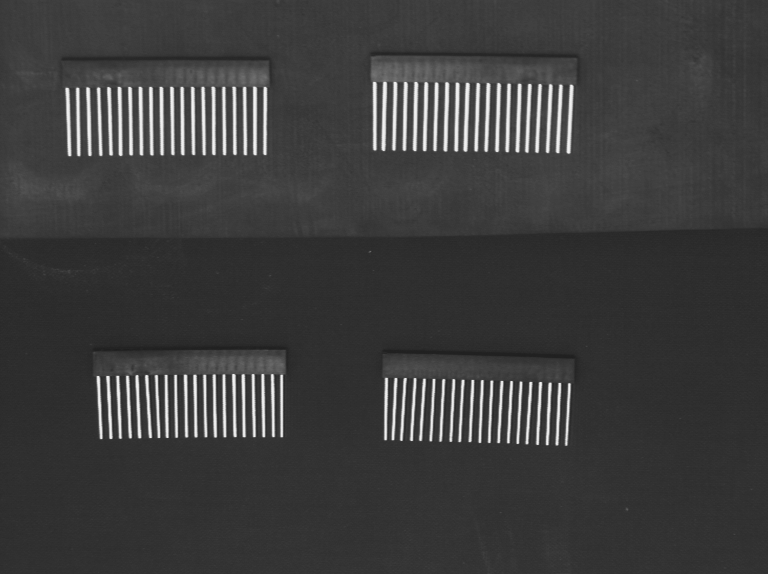
\includegraphics[scale=0.5]{images/ConnectOK.png}\hfill
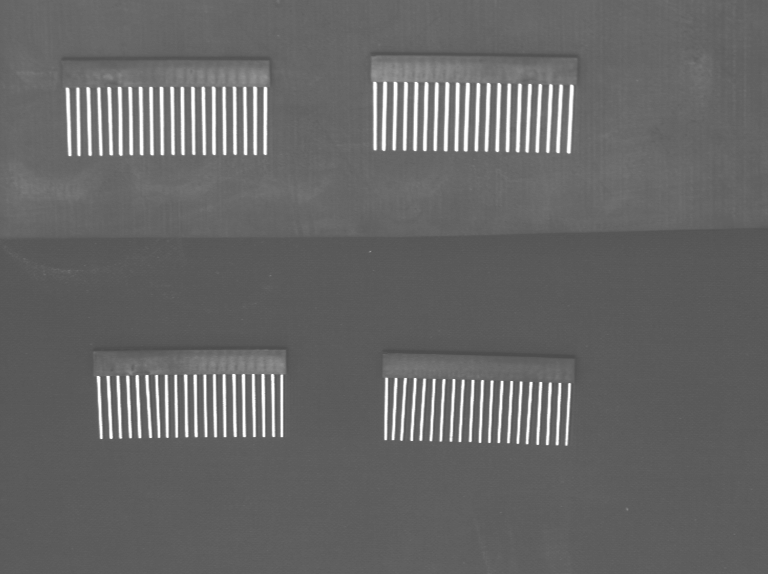
\includegraphics[scale=0.5]{images/ConnectL.png}\hfill
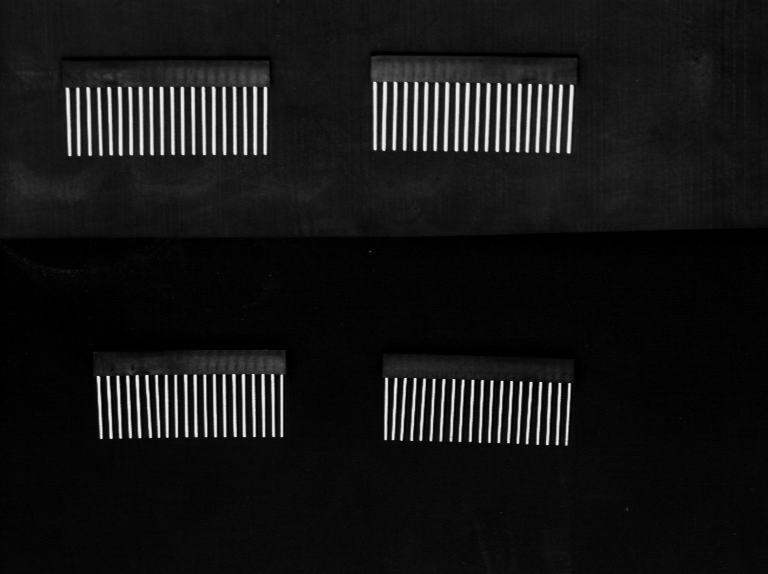
\includegraphics[scale=0.5]{images/ConnectD.png}
\caption{Connect Ok L D }
\end{figure}
\begin{figure}[!h]
\centering
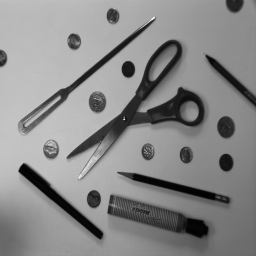
\includegraphics[scale=0.6]{images/PNCN256.png}
\caption{PNCN 256}
\end{figure}
\end{center}

\newpage
Tout d'abord, les images étant en niveaux de gris, nous avons commencé par effectuer les histogrammes des images de la figure 1.1. 
Sur cette figure sont présents l'histogramme de Connect_OK en bleu, de Connect_L en rouge et de Connect_D en vert. 
On constate de manière générale, que l'histogramme de la version "light" est décalé vers les niveaux de gris élevés par rapport
à l'histogramme de la version "OK" contrairement à celui de la version "dark" qui est décalé vers les niveaux de gris plus faibles.
Cela nous indique que l'image version "light" a été prise avec une forte luminosité comparé à celle lors de la prise de l'image "OK", 
contrairement à l'image version "dark" qui a été prise, quant à elle, avec une faible luminosité.
Grâce à l'outil Threshold, on a pu évaluer des encadrements de niveaux de gris pour chaque partie de ces images (voir table 1.1).
 
\begin{figure}[!h]
\centering
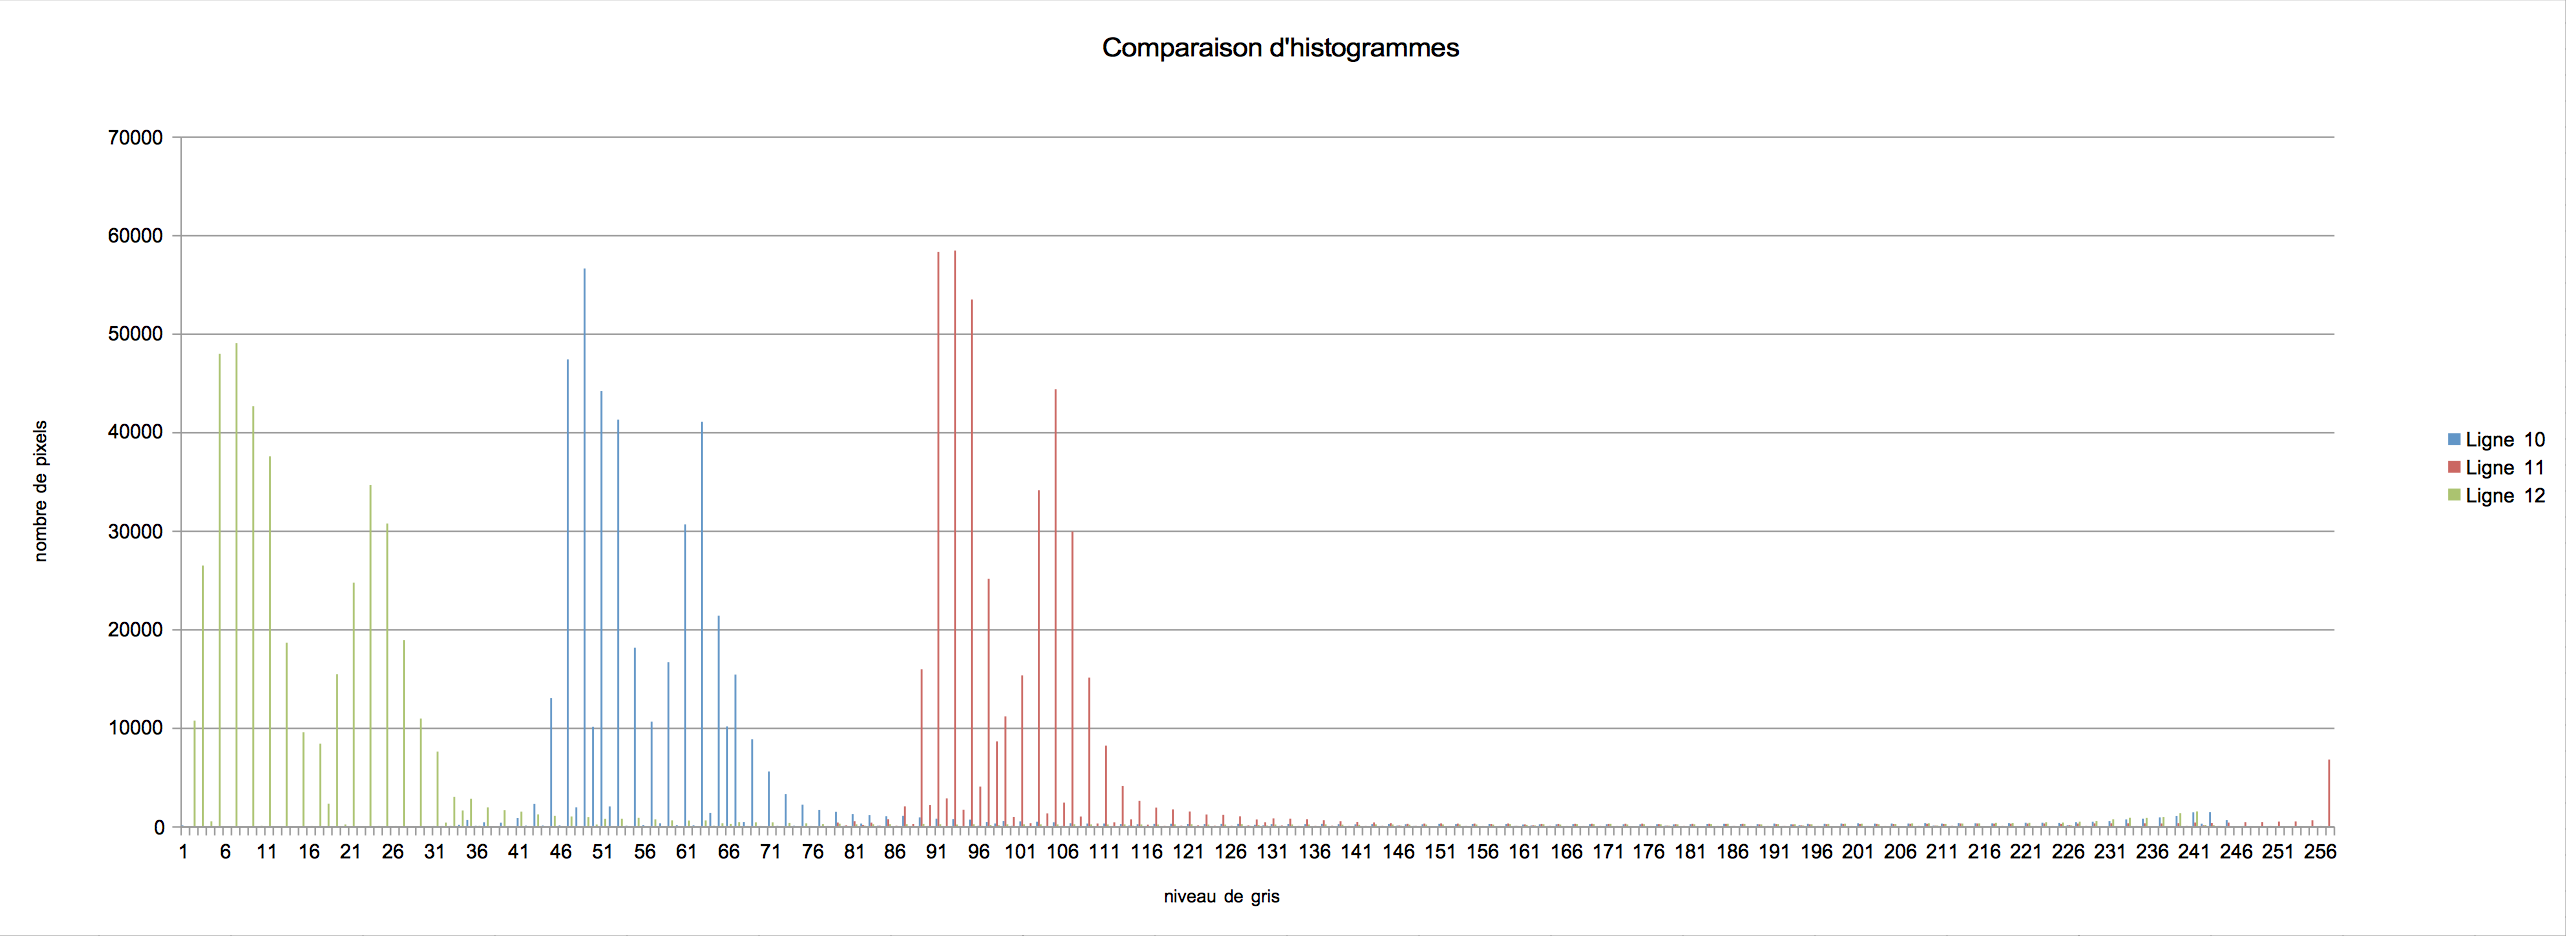
\includegraphics[width=15cm]{images/histogrammes1.png}
\caption{Histogrammes de Connect Ok L D}
\end{figure}

\begin{table}[!h]
	\begin{center}
		\begin{tabular}{|c|c|c|c|}
		   \hline
		   & Connect_D & Connect_OK & Connect_L \\
		   \hline
		   Les broches & [195,240]& [200,245] & [225,256]\\
		   \hline
		   Partie foncée & [0,76] & [30,116] & [76,161]\\
		   \hline
		\end{tabular}
	\end{center}
	\caption{Comparaisons : plage niveaux de gris}
\end{table}

\newpage
Sur les même images, nous avons également pris le temps de réaliser des comparaisons de profils de lignes. Le code couleur est le même
que pour les histogrammes. Nous avons pris soin d'augmenter le nombre d'échantillons pris pour les profils à 256 chacun. Chaque pic 
correspond à une broche. Le fait que les transitions fond/broche ne soient pas nettent est explicable soit par le fait que le nombre
d'échantillon (256 soit le maximum que l'on peut réaliser d'un point de vue technique ici) est insufisant soit par le fait que la résolution
du capteur qui a pris cette image n'est pas assez élevée.

\begin{figure}[!h]
\centering
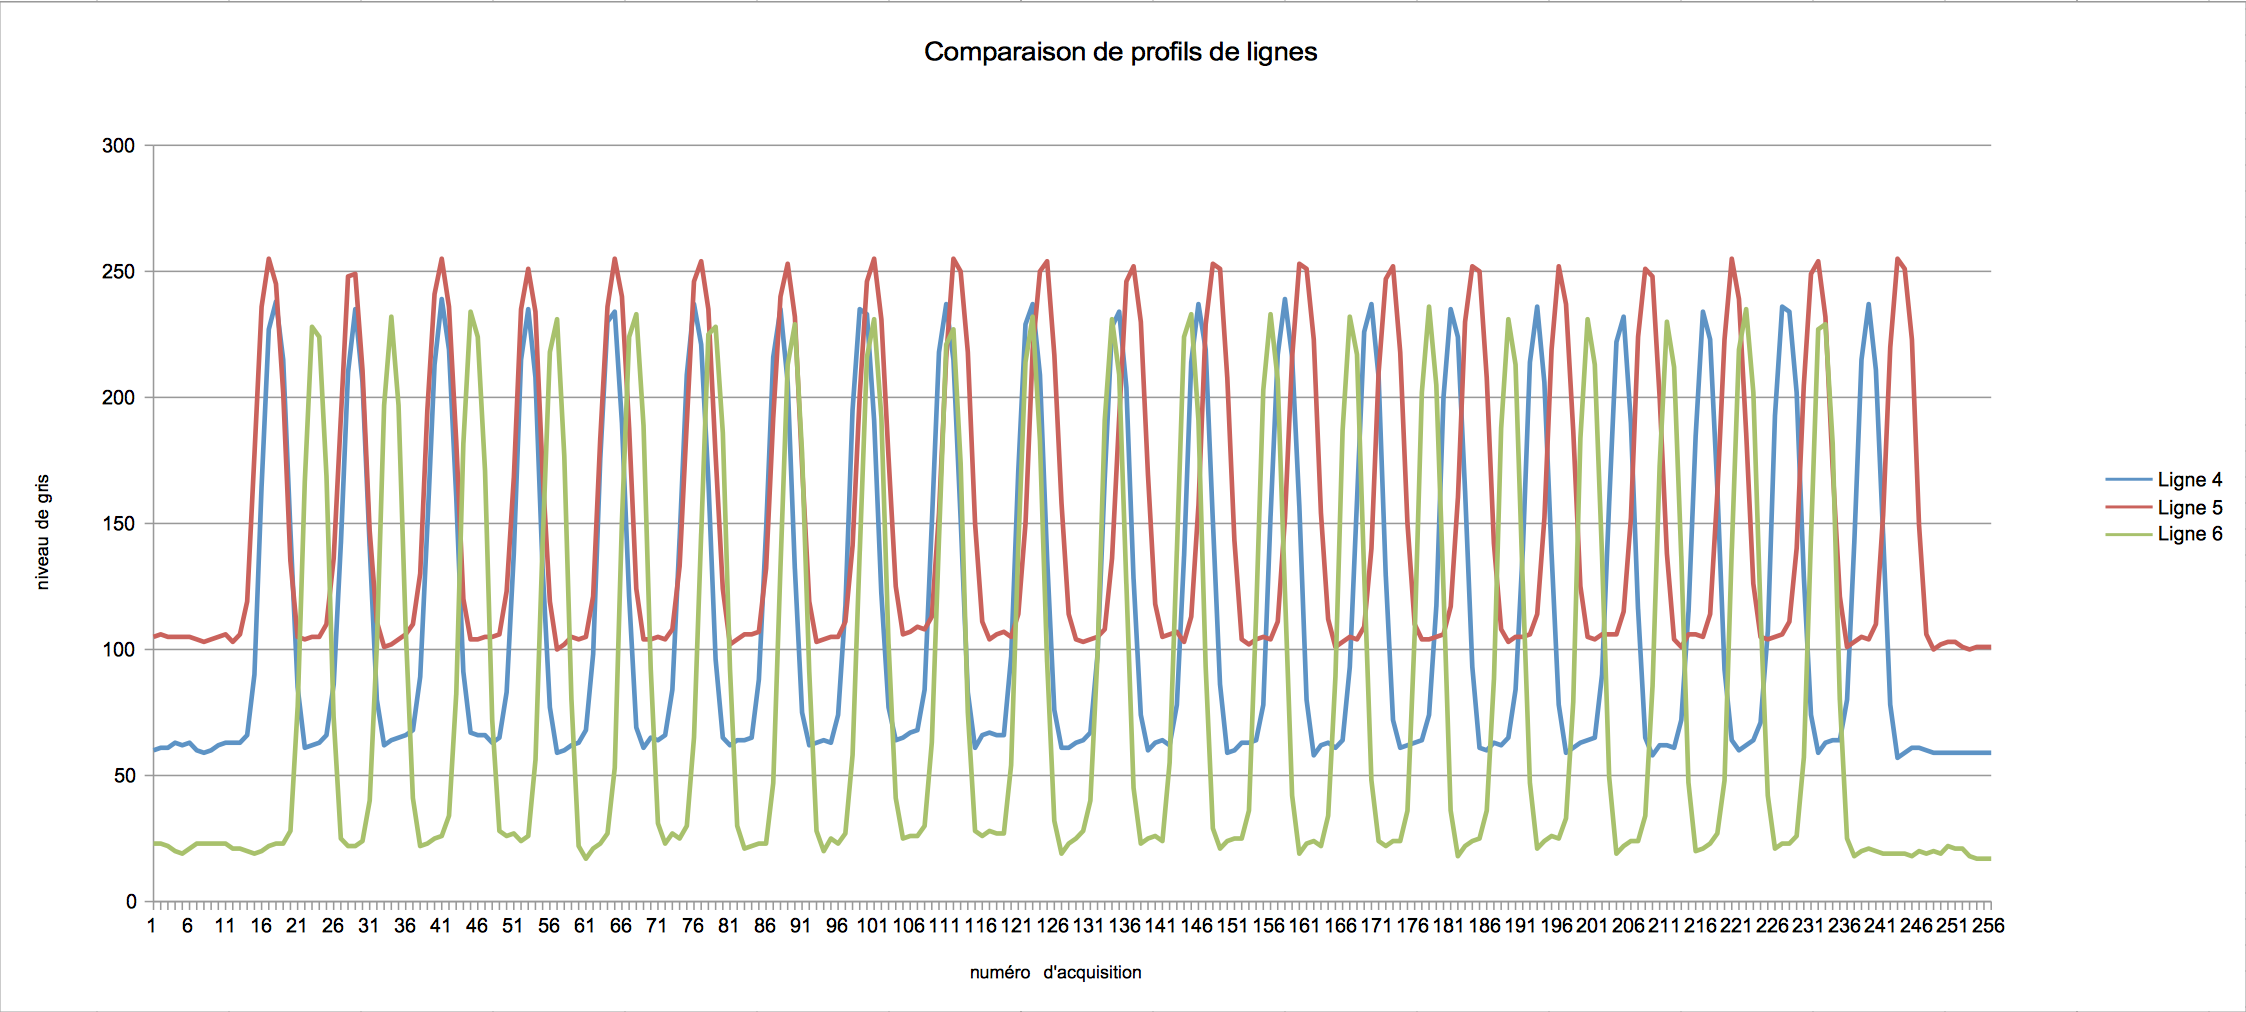
\includegraphics[width=15cm]{images/profildeligne1.png}
\caption{Profils de ligne de Connect Ok L D}
\end{figure}

\newpage
Maintenant, concentrons nous sur l'image PNCN256. Nous avons dans un premier temps réalisé l'histogramme de celle-ci. Nous observons que 
la dynamique de cette image s'étant du niveau de gris 0 au niveau de gris 200 environ. Il est difficile avec cet histogramme de séparer
les différents objets du fond. En effet, cet histogramme est plutôt condensé comparé à ceux des trois autres images déjà analysées. 
On peut remarquer maintenant après réalisation du profil de ligne du allant du coin haut gauche au coin bas droite de l'image, un problème 
d'éclairage de la scène. En effet, on a des niveaux de gris élevé du côté du coin haut gauche et des niveaux de gris plus faibles du côté 
du coin bas droite. Cela met en évidence un éclaire non homogène venant du coin haut gauche de l'image de la scène. 
  

\begin{figure}[!h]
\centering
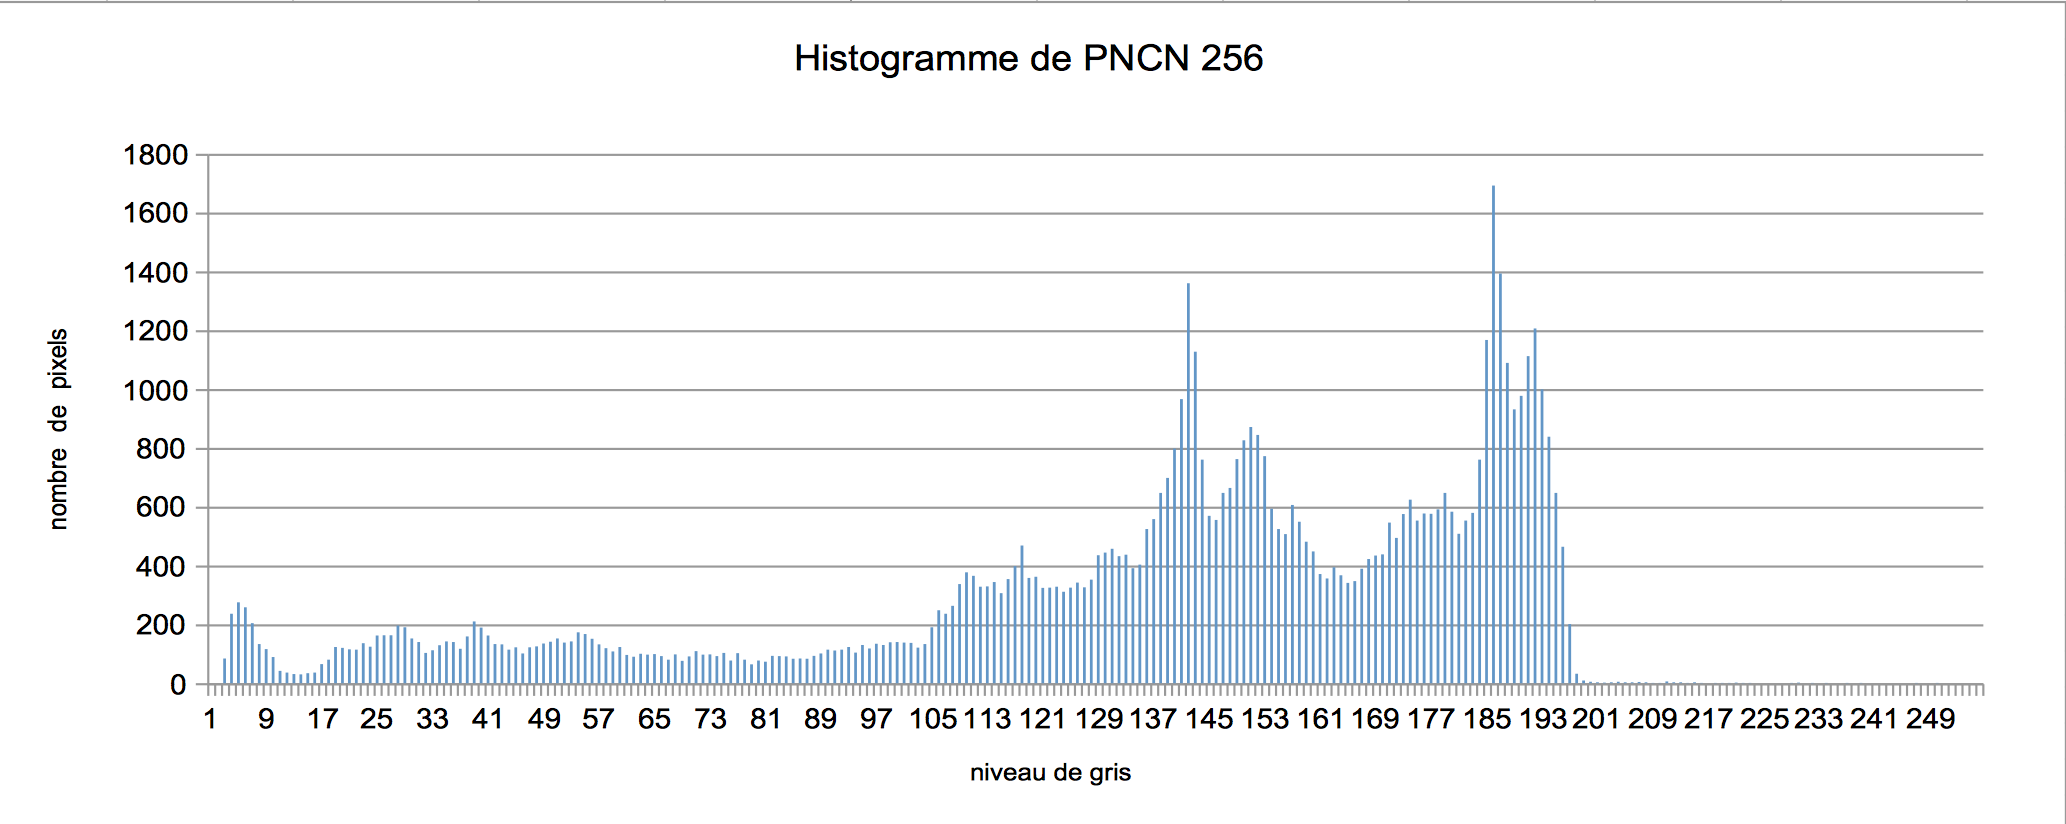
\includegraphics[width=15cm]{images/histogramme2.png}
\caption{Histogramme de PNCN 256}
\end{figure}

\begin{figure}[!h]
\centering
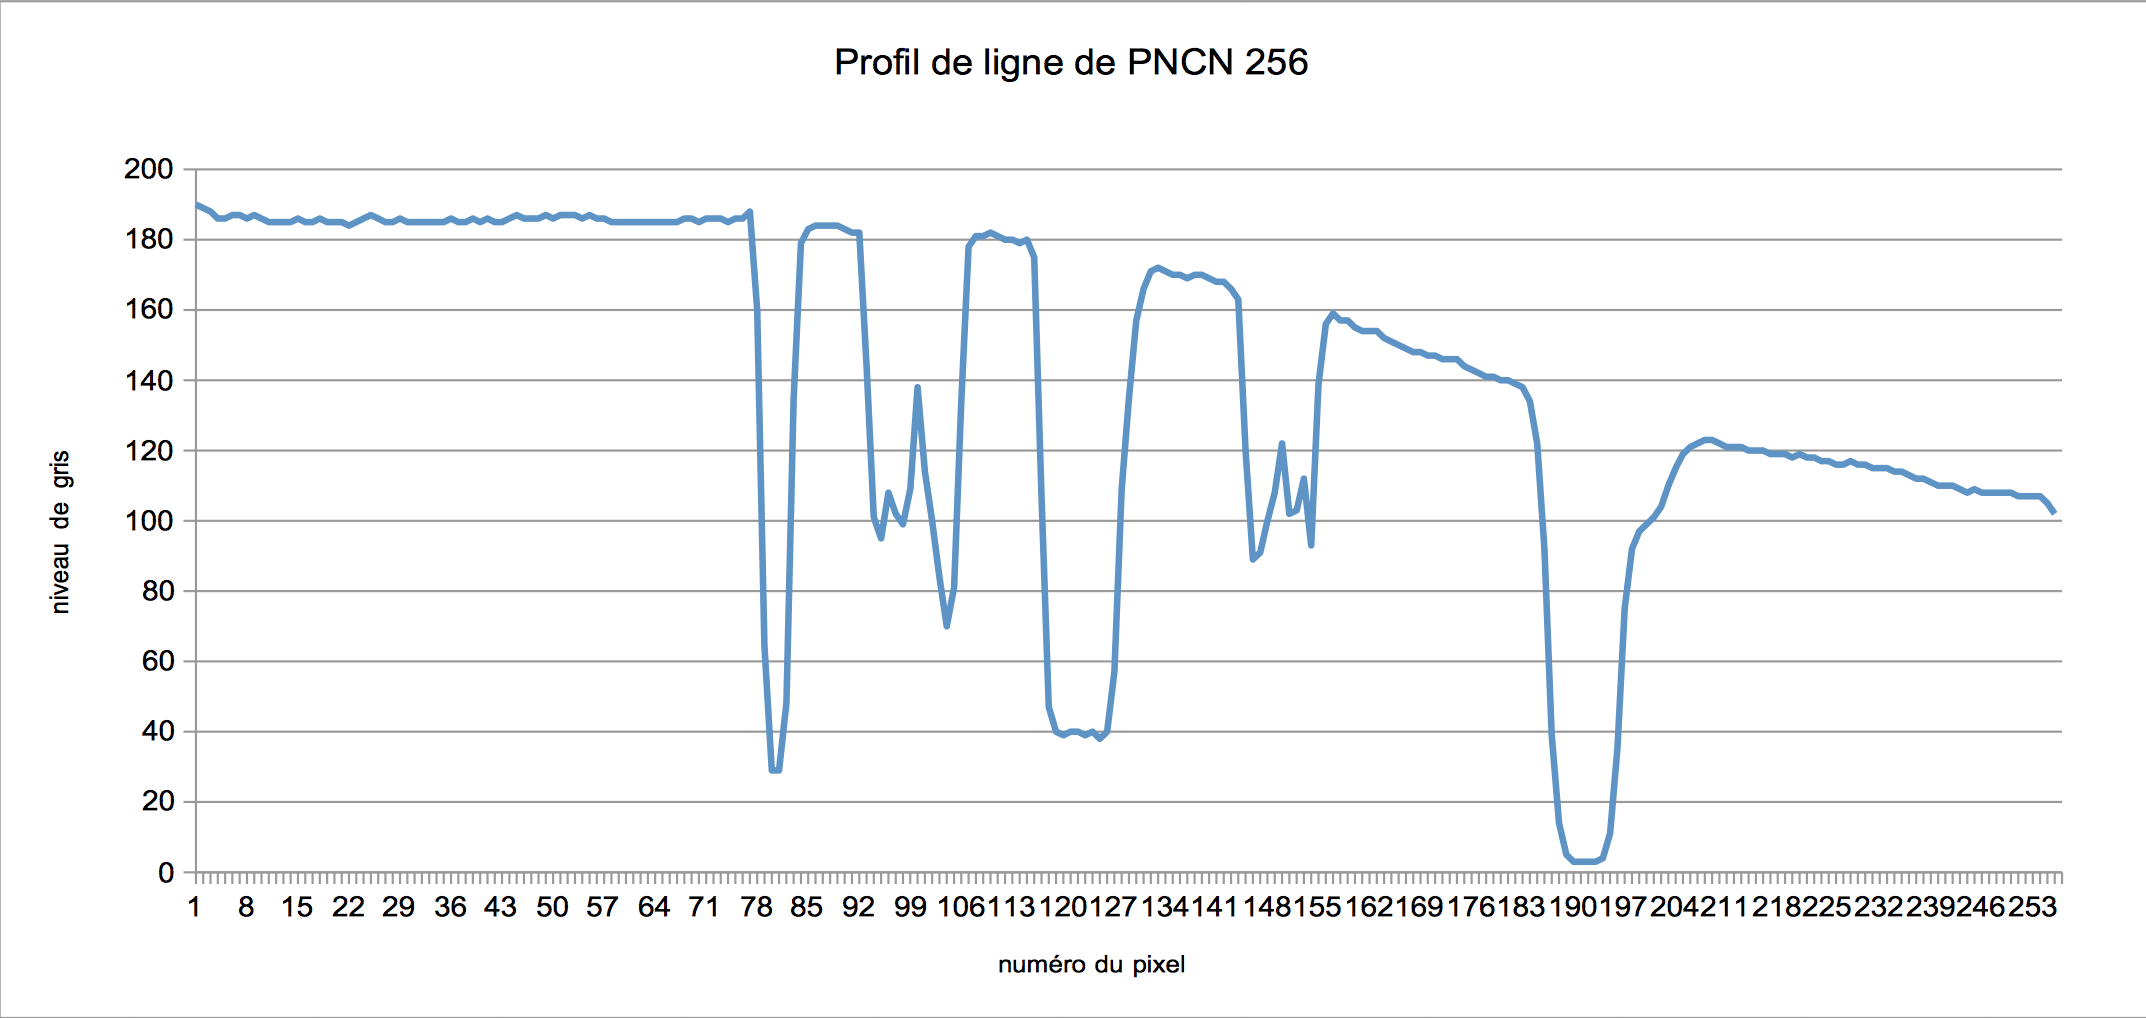
\includegraphics[height=5cm,width=15cm]{images/profildeligne2.png}
\caption{Profil de ligne de PNCN 256}
\end{figure}

\chapter{Deuxième Partie : Traitements aux environs du pixel}

\chapter{Troisième Partie : Filtrage Morphologique}

\end{document}

